% Method = arm B (field_pointwise + q_source=grad) as the headline;
% zeroth/tilted presented as dial instantiations evaluated in the ablation.
% Code refs: imitation/algos/dice/drift_field.py, distill_rl.py:field_actor_loss.

\Cref{sec:toy} left us with a concrete requirement: follow the critic where
it has data, and prevent the policy from wandering to where it does not.
Crucially, this is a requirement about \emph{where the policy ends up}, not
about how fast it travels --- a distinction the experiments turn out to
hinge on.

Where the critic stops being reliable is not something we can compute --- if
we could estimate its competence region we would already have solved the
problem --- so we approximate that boundary by the only landmark available:
the frozen policy the critic was trained around. Actions near its output the
critic has seen; actions far from it, it has not. The constraint therefore
takes the form of a radius about the base policy's own action.

\method{} --- \emph{Constrained Action-Space Transport} --- turns this into
an update rule. It \emph{transports} candidate actions toward higher critic
value, and it \emph{constrains} that transport \emph{in action space, on the
regression target, before anything is fitted}. The transport primitive
itself (move samples along a velocity field, regress the network onto the
moved samples) is inherited from the action-gradient family
\citep{dipo2024,psenka2024qsm}; the contribution is the constraint. Nothing
in the update needs a likelihood, a denoising objective, or the generator's
internals --- only a frozen noise-to-action map, $K$ samples from it, and a
critic --- so it applies unchanged across one-step, flow-matching and
diffusion policies (\cref{sec:exp-generality}).

\begin{figure}[t]
  \centering
  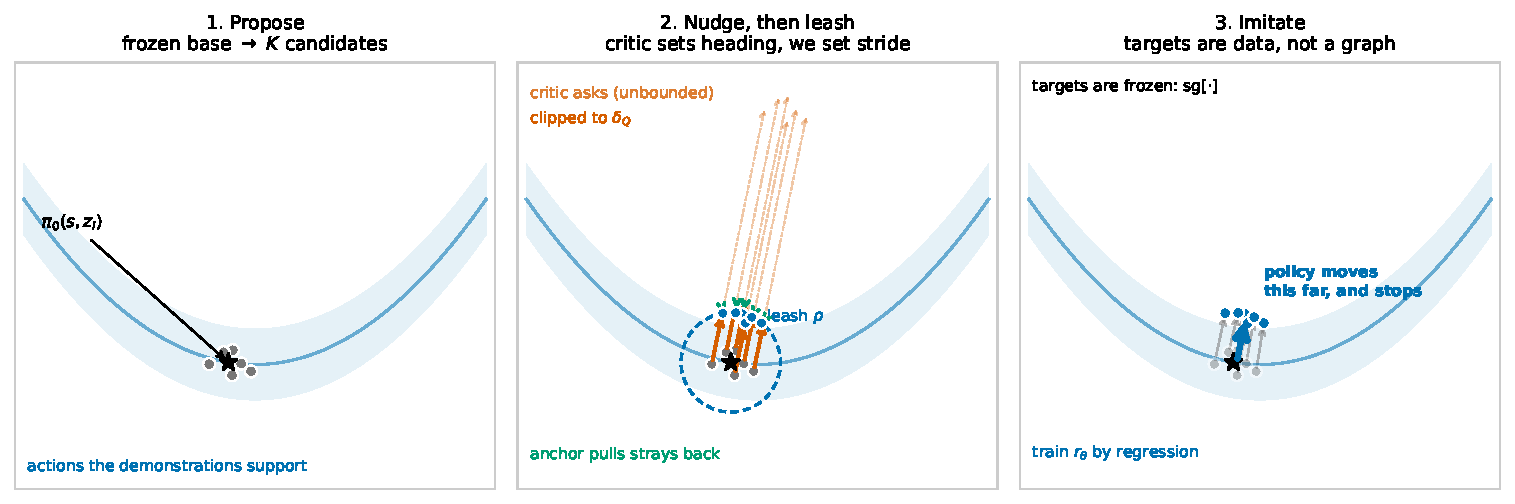
\includegraphics[width=\linewidth]{figures/method_overview.pdf}
  \caption{\textbf{\method{} in four steps} (schematic; one candidate drawn
  bold and followed through the pipeline). \textbf{(1)~Propose:} the frozen
  base maps $K$ noise samples to candidate actions on the band the
  demonstrations support. \textbf{(2)~Nudge:} the critic's raw ask points far
  off that band (dashed); \method{} keeps only its direction and steps at most
  $\delta_Q$ (solid). \textbf{(3)~Leash:} candidates that end up outside the
  dead zone of radius $\rho$ around the base action are pulled back to its
  rim (green); those inside are left alone --- the interior is free.
  \textbf{(4)~Imitate:} the corrected targets are detached
  ($\mathrm{sg}[\cdot]$) and the residual head is regressed onto them; no
  critic gradient ever backpropagates into the policy. The base is any frozen
  noise-to-action map.}
  \label{fig:method}
\end{figure}

\subsection{\method{} in four steps}
\label{sec:field-update}

The critic's answer is treated as advice about \emph{direction}; how far to
act on it is our choice, and the critic is never differentiated through. One
update does four things:

\begin{enumerate}
  \item \textbf{Propose.} Draw $K$ noise samples and push them through the
  frozen base plus the current residual, giving $K$ candidate actions for this
  state.
  \item \textbf{Nudge.} Ask the critic which direction improves each
  candidate, and take a step of bounded length in that direction --- the
  critic sets the heading, we set the stride.
  \item \textbf{Leash.} If a candidate has drifted more than $\rho$ away from
  what the frozen policy proposed, pull it back toward that action. Inside
  $\rho$ nothing happens, so the critic has free rein where it is trustworthy.
  \item \textbf{Imitate.} Detach the corrected candidates and train the
  residual head by regression onto them. They are data now, not a computation
  graph.
\end{enumerate}

Two consequences are worth noticing immediately. Because step 4 is plain
regression onto fixed targets, the size of the parameter update is set by us,
not by how steep the critic happens to be. And because step 3 measures distance
from the \emph{frozen} policy rather than from the previous iterate, the
reference point never moves --- which, as \cref{sec:exp-constraint} shows, is
exactly what separates a constraint that works from one that does not.

Concretely: for each state in the batch we draw $K$ noise samples and form the
current action candidates $a_i = \pi_0(s, z_i) + r_\theta(s, z_i)$, treated as
constants (detached). Each is displaced by a combined velocity,
\begin{equation}
  \tilde{r}_i \;=\; \mathrm{sg}\!\left[\, r_i
     \;+\; \operatorname{clip}_{\delta_Q}\!\big(V_Q(s, z_i, a_i)\big)
     \;+\; V_{\mathrm{anc}}(r_i) \,\right],
  \qquad
  \mathcal{L}_{\mathrm{actor}}
  = \frac{1}{K}\sum_i \big\| r_\theta(s, z_i) - \tilde{r}_i \big\|^2 ,
  \label{eq:update}
\end{equation}
where $\mathrm{sg}[\cdot]$ is stop-gradient and
$\operatorname{clip}_{\delta}(v) = v \cdot \min(1, \delta / \|v\|)$
rescales a field vector to norm at most $\delta$.

Matching this to the four steps: $V_Q$ is the critic's direction (step 2),
clipped to length $\delta_Q$; $V_{\mathrm{anc}}$ is the leash (step 3),
silent while $\|r_i\|$ stays within $\rho$; the total displacement is clipped
to $\delta_{\mathrm{tot}}$; and $\mathrm{sg}[\cdot]$ makes the result a fixed
regression target (step 4). The critic is trained separately
(\cref{sec:critic}). \Cref{tab:design} collects every design choice, its
role, and the value we run.

\begin{table}[t]
\centering
\caption{\textbf{\method{}'s parts, and how each is designed.} One row per
component of \cref{eq:update}. Defaults are the family-shared recipe
(LIBERO); robomimic differs only where noted. Each part's sensitivity is
measured in the referenced experiment.}
\label{tab:design}
\small
\resizebox{\linewidth}{!}{%
\begin{tabular}{llllc}
\toprule
component & role & design & default & ablated in \\
\midrule
candidates $K$ & coverage of the base's action modes & noise samples through the frozen base $+$ residual & $16$ & \cref{tab:resolution} \\
reward field $V_Q$ & \emph{direction} of improvement & normalized critic gradient $\eta_Q \nabla_a \bar Q / q_{\mathrm{scale}}$ & $\eta_Q{=}1$ ($0.5$ robomimic) & \cref{tab:eta-sweep} \\
step clip $\delta_Q$, $\delta_{\mathrm{tot}}$ & \emph{stride}: caps each displacement & rescale to norm at most $\delta$ & $\delta_{\mathrm{tot}}{=}0.15$ & \cref{tab:constraint} \\
anchor $V_{\mathrm{anc}}$ & keeps targets near the base & dead-zone restoring field, \cref{eq:anchor} & $\eta_{\mathrm{anc}}{=}1$ & \cref{tab:constraint} \\
dead zone $\rho$ & region where the critic is trusted freely & radius about the base action ($\rho{=}0$ = always-on pull) & $0.05$ rms (LIBERO); $0$ (robomimic, DMC) & \cref{tab:rho-sweep} \\
regression (\cref{eq:update}) & converts targets into parameters & MSE onto detached targets; no critic gradient & --- & \cref{tab:matched} \\
\bottomrule
\end{tabular}}
\end{table}

\paragraph{Why displace targets rather than differentiate.} Writing the
update as regression onto displaced targets is what makes the boundary
enforceable at all. The quantity we need to bound --- how far the policy's
action ends up from the base policy's action --- is a property of the
\emph{target}, and here it is available explicitly, before any gradient is
taken: we can inspect each displaced target, compare it to the action it came
from, and correct it. Backpropagating $-Q$ offers no such handle, because the
distance travelled is an emergent consequence of a parameter step and is not
represented anywhere the algorithm can act on. Two secondary properties follow
from the same choice. The regression target is detached, so the critic never
differentiates through the actor and cannot inject unbounded curvature into
the parameter update. And because targets are formed from freshly drawn
samples rather than from stored actions rewritten in place, replayed
transitions continue to describe the dynamics that produced them --- a
consistency DIPO's buffer rewrite gives up
\citep{dipo2024}.

\paragraph{What the clip does and does not guarantee.}
The clip bounds \emph{target transport}, and only that:
\begin{equation}
  \|\tilde r_i - r_i\| \;\le\; \delta_{\mathrm{tot}}
  \qquad\text{for every particle } i .
  \label{eq:target-bound}
\end{equation}
It is tempting to read this as a bound on how far the \emph{policy} moves,
and an earlier version of this work did. That inference is invalid. The
targets are amortized through a shared network by a gradient step, so to
first order the realized change at particle $i$ is
\begin{equation}
  \Delta r_i \;\approx\; \alpha \sum_j J_i J_j^{\top}\,(\tilde r_j - r_j),
  \qquad J_i = \partial r_\theta(s,z_i)/\partial\theta ,
  \label{eq:ntk-coupling}
\end{equation}
and the Jacobian coupling across particles carries no guarantee that
$\|\Delta r_i\| \le \delta_{\mathrm{tot}}$. This is precisely the
objection we raise against parameter-space gradient clipping
(\cref{sec:failure-modes}), and it applies to target-space clipping too:
bounding what the network is \emph{asked} for does not bound what it
\emph{does}. A per-particle guarantee would require an output-space proximal
step, exact interpolation, or a tabular actor --- none of which we impose.

The distinction matters, but it does not undermine the construction, because a
per-particle guarantee is not what the update needs. A drift assembled from
many individually permitted steps is still a drift, since the critic keeps
pointing the same way and nothing returns the policy --- which is why the
constraint that matters is one whose strength grows with the displacement
already accumulated, rather than one that merely rate-limits each step. What
we establish empirically is narrower and sufficient: with no action-space
bound of any kind the update destroys the policy, and with either bound
present it does not (\cref{sec:exp-constraint}).

\subsection{The reward field $V_Q$}
\label{sec:reward-field}

The default (and headline) reward field is the normalized critic
gradient evaluated at each particle,
\begin{equation}
  V_Q^{\mathrm{grad}}(s, z, a)
  \;=\; \eta_Q \, \frac{\nabla_a \bar{Q}_\phi(s, z, a)}{q_{\mathrm{scale}}},
  \qquad q_{\mathrm{scale}} = \mathbb{E}\big[\,|\bar{Q}_\phi|\,\big],
  \label{eq:vq-grad}
\end{equation}
where $\bar{Q}_\phi$ is the conservative ensemble aggregate. This is
deliberately the \emph{same scalar} the DICE-RL actor optimizes: in the
small-step, unclipped limit, minimizing \cref{eq:update} recovers the
backpropagated update direction exactly (\cref{prop:equiv}), so any
performance difference is attributable to the update form --- the anchored
target regression --- and not to a different reward signal.

\paragraph{The kernel transport operator.} The lower-resolution reward
fields below and the distributional anchor variant share one particle
transport operator, which we take off the shelf \citep{deng2026drifting}; it
is a convenience for turning a set of target particles into a velocity field,
and nothing in the method depends on its particular form. Given query particles $x$, attractor particles
$p^{+}$ (optionally weighted), and repulsor particles $p^{-}$, distances are
normalized by a global scale and, for each kernel radius $R$ in a small set,
a soft mutual-matching affinity
$A = \sqrt{\mathrm{softmax}_{\mathrm{row}}(-d/R) \odot
\mathrm{softmax}_{\mathrm{col}}(-d/R)}$ converts matched attractors into
pulls and matched repulsors into pushes; forces are summed over radii to
give $\mathcal{V}(x \mid p^{+}, p^{-})$ (full form in
\cref{app:kernel}). Intuitively, $\mathcal{V}$ moves a particle cloud so
its density flows toward $p^{+}$ and away from $p^{-}$ --- it needs only
\emph{samples} of the target, never a density or a gradient.

Because $V_Q$ enters \cref{eq:update} only as a velocity, the critic
can be consumed at \emph{lower resolution} when its gradients are not
trustworthy, using only $Q$-values:
\begin{itemize}
  \item \textbf{zeroth-order (top-$k$):} rank the $K$ particles by
  $Q$ and set $V_Q = \mathcal{V}(a \mid \text{top-}k \text{ particles},
  \text{all particles})$ --- the pretraining kernel transport toward
  the critic's preferred candidates;
  \item \textbf{tilted:} let every particle attract with weight
  $K\cdot\mathrm{softmax}_i(\mathrm{adv}_i/\tau)$, transporting the
  cloud toward its own $\exp(Q/\tau)$-tilted density, the canonical
  improvement target of \citet{peng2019awr,abdolmaleki2018mpo}.
\end{itemize}
These are not competing methods but settings of a dial --- how much of
the critic's local structure the update trusts: full first-order
information, ranking only, or soft value weights. \Cref{sec:experiments}
maps the regimes: the gradient source dominates wherever the critic
generalizes, while the value-only sources close the gap precisely in
the weak-critic regime predicted by \cref{sec:toy}.

\subsection{The anchor field}
\label{sec:anchor}

The kernel reward fields vanish beyond their largest radius and the
gradient field carries no notion of the data manifold, so
\cref{eq:update} alone would let the residual random-walk. The anchor
is a \emph{restoring} field with a dead zone,
\begin{equation}
  V_{\mathrm{anc}}(r) \;=\; -\,\eta_{\mathrm{anc}}
  \left(1 - \frac{\rho}{\|r\|}\right)_{\!+} r ,
  \label{eq:anchor}
\end{equation}
which is inert inside the trust radius $\rho$ and pulls back only the
excess residual norm beyond it. Equivalently, \cref{eq:anchor} is the
negative gradient of a hinged radial potential,
\begin{equation}
  U(r) \;=\; \tfrac{1}{2}\,\eta_{\mathrm{anc}}\big(\|r\| - \rho\big)_{+}^{2},
  \qquad V_{\mathrm{anc}}(r) \;=\; -\nabla_r U(r),
  \label{eq:anchor-potential}
\end{equation}
so it removes exactly the radial excess and nothing else. Setting $\rho = 0$
gives $U(r) = \tfrac{1}{2}\eta_{\mathrm{anc}}\|r\|^{2}$ --- the quadratic
residual regularizer of the backpropagated control --- so the dead zone is a
hinge generalization of that penalty, with $\rho$ interpolating between them. Unlike a $\lambda\|r\|^2$ penalty ---
which competes with an unbounded gradient and loses
(\cref{sec:toy}) --- \cref{eq:anchor} composes with the clipped reward
field as a velocity, so the residual scale is set geometrically rather than
by a loss-weight arms race. Heuristically, if the reward field were
stationary, radially outward and saturated at $\|V_Q\| = \delta_Q$, balancing
it against the anchor outside the dead zone gives
$\delta_Q = \eta_{\mathrm{anc}}(\|r\| - \rho)$, i.e.\ $\|r\| = \rho +
\delta_Q/\eta_{\mathrm{anc}}$. We use this only as a scale estimate when
choosing $\eta_{\mathrm{anc}}$: a learned critic's field varies in direction
and magnitude with $r$, so there may be several fixed points, cycles, or
none, and we claim no unique equilibrium.

\subsection{Relation to the backpropagated actor; critic}
\label{sec:critic}

\begin{proposition}[Small-step equivalence]
\label{prop:equiv}
At the current parameters, the gradient of \cref{eq:update} is
$\nabla_\theta \mathcal{L}_{\mathrm{actor}} \propto
-\big(\operatorname{clip}_{\delta_Q}(V_Q) + V_{\mathrm{anc}}\big)^{\!\top}
\partial r_\theta / \partial \theta$. With
$V_Q = V_Q^{\mathrm{grad}}$, no clipping
($\delta_Q, \delta_{\mathrm{tot}} \to \infty$) and $\rho = 0$, this is
the DICE-RL residual actor gradient with anchor weight
$\eta_{\mathrm{anc}}$.
\end{proposition}

\method{} is therefore a strict generalization of its control: the new
degrees of freedom are the pointwise action-space clip, the dead-zone
anchor, and the resolution dial on $V_Q$ --- each of which we ablate.

\emph{Remark (not just clipped gradient ascent).} One might object that
\cref{eq:update} with $V_Q^{\mathrm{grad}}$ is ``DDPG with clipping.''
The distinction is where the bound lives. Clipping $\nabla_\theta$ bounds a
\emph{parameter} step, whose effect on the policy output is unknown and
state-dependent; \cref{eq:update} bounds the \emph{policy's motion at every
particle}, which is the quantity that off-manifold failure depends on
(\cref{sec:toy}). Moreover, only the regression form makes the two other
components expressible at all: a dead-zone anchor and a value-only $V_Q$
have no loss-gradient counterpart. The ablations in
\cref{sec:exp-locus} test each distinction in isolation.
The critic is unchanged from DICE-RL: ensemble TD with a CQL-style
penalty pushing $Q$ down at policy actions and up at data actions;
field construction never leaks gradients into the critic
(gradients w.r.t.\ actions only). \Cref{alg:cast} summarizes one joint
update.

\begin{algorithm}[t]
\caption{\method{}: one update ($V_Q^{\mathrm{grad}}$ variant)}
\label{alg:cast}
\begin{algorithmic}[1]
\Require frozen base $\pi_0$; residual $r_\theta$; critic $Q_\phi$;
  steps $\eta_Q, \eta_{\mathrm{anc}}$; clips $\delta_Q, \delta_{\mathrm{tot}}$;
  dead zone $\rho$; particles $K$
\State sample batch of states $s$; draw $z_i \sim \mathcal{N}(0, I)$,
  $\;a_i \gets \pi_0(s, z_i) + r_\theta(s, z_i)$ \Comment{no grad}
\State $V_i \gets \operatorname{clip}_{\delta_Q}\!\big(\eta_Q\,
  \nabla_{a}\bar{Q}_\phi(s, z_i, a_i) / q_{\mathrm{scale}}\big)$
  \Comment{or top-$k$ / tilted kernel field}
\State $V_i \gets V_i - \eta_{\mathrm{anc}}
  \big(1 - \rho / \lVert r_i \rVert\big)_{+}\, r_i$
  \Comment{dead-zone anchor, \cref{eq:anchor}}
\State $\tilde{r}_i \gets \mathrm{sg}\big[\, r_i +
  \operatorname{clip}_{\delta_{\mathrm{tot}}}(V_i) \,\big]$
  \Comment{policy moves $\leq \delta_{\mathrm{tot}}$, always}
\State $\theta \gets \theta - \alpha\, \nabla_\theta \tfrac{1}{K}
  \textstyle\sum_i \lVert r_\theta(s, z_i) - \tilde{r}_i \rVert^2$
\State update $\phi$: ensemble TD + CQL penalty \Comment{unchanged from
  \citet{dicerl2026}}
\end{algorithmic}
\end{algorithm}
